\documentclass[tikz,border=10pt]{standalone}
\usepackage{amsmath}
\begin{document}
\begin{document}
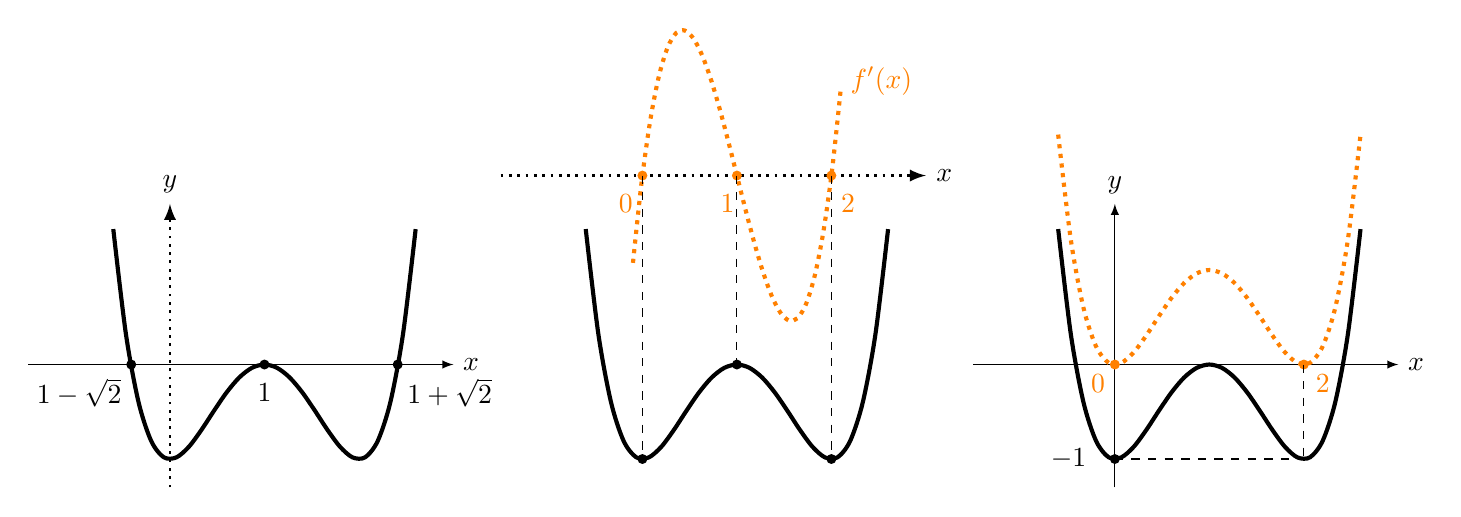
\begin{tikzpicture}[scale=1.2]
	%1
    \draw[-latex] (-1.5,0) -- (3,0) node[right] {$x$};
    \draw[-latex, dotted, line width=1pt] (0,-1.3) -- (0,1.7) node[above] {$y$};
    
    \draw[smooth, line width=1.5pt] plot[domain=-0.6:2.6] (\x,{(\x)^2*(\x-2)^2-1});
    
	\node at (-0.41,-0.3) [left] {$1-\sqrt2$};
	\node at (1,-0.1) [below] {$1$};
	\node at (2.41,-0.3) [right] {$1+\sqrt2$};

	\fill (-0.41,0) circle (1.5pt);
	\fill (1,0) circle (1.5pt);
	\fill (2.41,0) circle (1.5pt);

	%2
	\begin{scope}[shift={(5,0)}]

    \draw[-latex,dotted,line width=1pt] (-1.5,2) -- (3,2) node[right] {$x$};
    
    \draw[smooth, orange, dotted, line width=1.5pt] plot[domain=-0.1:2.1] (\x,{4*\x*(\x-1)*(\x-2)+2});
    \draw[smooth, line width=1.5pt] plot[domain=-0.6:2.6] (\x,{(\x)^2*(\x-2)^2-1});
    
	\node[orange] at (0,1.7) [left] {$0$};
	\node[orange] at (0.9,1.9) [below] {$1$};
	\node[orange] at (2,1.7) [right] {$2$};
	\node at (2.1,3) [right, orange] {$f'(x)$};

	\fill[orange] (0,2) circle (1.5pt);
	\fill[orange] (1,2) circle (1.5pt);
	\fill[orange] (2,2) circle (1.5pt);

	\fill (0,-1) circle (1.5pt);
	\fill (1,0) circle (1.5pt);
	\fill (2,-1) circle (1.5pt);

	\draw[dashed] (0,2) -- (0,-1);
	\draw[dashed] (1,2) -- (1,0);
	\draw[dashed] (2,2) -- (2,-1);

	\end{scope}

	%3
	\begin{scope}[shift={(10,0)}]
	
	\draw[-latex] (-1.5,0) -- (3,0) node[right] {$x$};
    \draw[-latex] (0,-1.3) -- (0,1.7) node[above] {$y$};
    
    \draw[smooth, orange, line width=1.5pt, dotted] plot[domain=-0.6:2.6] (\x,{(\x)^2*(\x-2)^2});
    \draw[smooth, line width=1.5pt] plot[domain=-0.6:2.6] (\x,{(\x)^2*(\x-2)^2-1});
    
	\node[orange] at (0,-0.2) [left] {$0$};
	\node[orange] at (2.2,0) [below] {$2$};
	\node at (-0.2,-1) [left] {$-1$};

	\fill[orange] (0,0) circle (1.5pt);
	\fill[orange] (2,0) circle (1.5pt);
	\fill (0,-1) circle (1.5pt);
	
	\draw[dashed] (2,0) -- (2,-1);
	\draw[dashed] (0,-1) -- (2,-1);
	
	\end{scope}
	  
\end{tikzpicture}
\end{document}
\end{document}